% \documentclass[12pt]{mitthesis} 
% \usepackage[pdftex]{graphicx}
% \usepackage{kylesthesis}
% \begin{document}

% \tableofcontents
% \clearpage

% \subsubsection*{NOTES}

% This is the third chapter of my thesis, essentially a final draft.  It
% follows the introduction chapter and the ``Models'' chapter (you
% have already seen the latter).

% A couple small changes still to be made: a long list of references in
% the second paragraph, and changing the lines below the spectrum to
% arrows in Figures 2 and 3.

% I am looking especially for any big changes that should be made --
% additional topics to include, sections to drop, or points to make more
% clear.

% I have also recently discovered two more examples of the use of
% deconvolution for doorway-coupling schemes, for propyne and
% methyl-vinyl-ether [Cupp, JCP 109, 4302 (1998); Go, JCP 97, 6994
% (1992)].  In both cases, the bright$\sim$doorway coupling is so strong
% that it splits the spectrum into two distinct clumps, which can be
% analyzed separately.  I think this provides a great example of the
% strong coupling case described in the ``Models'' chapter.  I will also
% mention these papers in the paragraph where I discuss previous efforts
% to take deconvolution beyond the direct-coupling model.\\

% --Kyle

% \clearpage
% \setcounter{chapter}{2}
\chapter{Deconvolution of spectral data to produce a doorway-coupling
  model Hamiltonian}

\section{Introduction}

Spectral deconvolution is a method of local deperturbation for
high-resolution spectroscopy, used to determine the parameters that
define a model Hamiltonian from an absorption spectrum.  The model
Hamiltonian determined by spectral deconvolution contains a single
zero-order bright state, which interacts with a set of
pre-diagonalized dark basis states.  Such a direct-coupling
Hamiltonian is shown in Figure \ref{fig:matrix}a.  In its discrete
formulation, spectral deconvolution returns a set of dark state
energies and squared bright$\sim$dark matrix elements.  In its
continuous formulation, the procedure returns a zero-order spectral
density function for coupling to the bright state.

Spectral deconvolution has been used to study Intramolecular
Vibrational Redistribution (IVR) in many small molecules, including
\ce{NO2}, allene, and several substituted propynes \cite{cable80,
  timmermans95, andrews98, hudspeth98}.  It was originally developed
in the study of intersystem crossing, where it has been used on the
spectra of intermediate case molecules such as acetylene, napthalene,
and pyrazine \cite{drabbels94, cable80, lawrance85}.

The technique for deconvolution of continuous spectra was described by
Berg and independently, in a more general form, by Ziv and Rhodes
\cite{berg76, ziv76}.  Both methods make use of a Green's function
formalism.  The discrete formulation of spectral deconvolution was
presented by Lawrance and Knight, and afterward simplified by Lehmann
\cite{lawrance85, lehmann91}.  Lehmann's refinement of the technique
obviates the need to compute any Green's function from the spectrum --
we refer to this method as Lawrance-Knight-Lehmann (LKL)
deconvolution.  Interestingly, the LKL method had been used in 1977 by
Brand and Hoy to deperturb portions of the \ce{NO2} spectrum
\cite{brand77}.  That work was cited by Cable and Rhodes, who
artificially re-broadened the same spectrum to demonstrate their
continuous deconvolution technique \cite{cable80}.

% The ultimate purpose of spectral deconvolution is to transform
% experimental information, the energies and spectral intensities of
% eigenstates, into an appropriate zero-order basis.  Although the
% zero-order states obtained from deconvolution may not be equivalent to
% the conventional Born-Oppenheimer basis states of the molecule,
% through a clever choice of ``brightness'' they may be diagonal in some
% quantum number of interest, and may facilitate interpretation in terms
% of selection rules for that quantum number.  For example, consider the
% case of ISC between a lone singlet rovibronic level and several
% triplet levels.  The spin selection rule $\Delta S=0$ for optical
% transitions ensures the unique ``brightness'' of the singlet level in
% transitions from a singlet ground state.  Upon deconvolution of the
% spectrum, the spin selection rule provides a natural separation in the
% resulting basis set according to the spin quantum number ($S=0$ for
% the bright state and $S=1$ for all dark states).  However, triplet
% sublevels belonging to different electronic states remain mixed (are
% not distinguished) in the basis provided by deconvolution.

The set of dark states available from LKL deconvolution loses its
lustre when an interaction of interest occurrs within the set of dark
states.  This is the case for sequential coupling among tiers of dark
states, a common situation in small polyatomic molecules
\cite{tramer05}.  Although dark state$\sim$dark state interactions
play a central role in the redistribution of molecular energy, the
deconvolution procedure does not directly yield information pertaining
to their dynamics.

To this end, several efforts have been made to investigate
perturbations within the block of pre-diagonalized dark states
returned by LKL deconvolution.  Pate, Lehmann, and Scoles used a
method of matrix rotation to obtain a qualitative explanation of a
J-dependent Coriolis interaction between two dark states in their
deperturbation of the trifluoropropyne spectrum \cite{pate91}.
Altunata and Field derived a parameter to predict the relative energy
of a single ``doorway'' state, a unique dark state that mediates all
coupling between the bright state and the remaining dark states
\cite{altunata01}.  A method to determine the energy and squared
matrix element of a doorway state from the spectrum allows the
construction of a new doorway-coupling model Hamiltonian.  Such a
Hamiltonian is shown in figure \ref{fig:matrix}b.

The parameters in a direct-coupling Hamiltonian are uniquely
determined by the spectrum; the total number of energies and
intensities in the spectrum is equal to the number of free parameters
in the model Hamiltonian.  For a spectrum consisting of $N+1$
transitions, the number of free parameters after normalization is
$2N+1$ ($N+1$ energies and $N$ normalized intensities)
\cite{lawrance85}.  A direct-coupling Hamiltonian contains $1$ bright
state energy, $N$ dark state energies, and $N$ bright$\sim$dark
coupling matrix elements, totaling $2N+1$.  A doorway-coupling
Hamiltonian also contains $2N+1$ free parameters: 1 bright state
energy, 1 bright$\sim$doorway matrix element, 1 doorway state energy,
$N-1$ dark state energies, and $N-1$ doorway$\sim$dark coupling matrix
elements.

The equal number of parameters in the direct and doorway-coupling
Hamiltonians suggests that a doorway-coupling Hamiltonian can also be
derived uniquely from the experimental data.  Such a technique was
described for the continuous case by Ziv and Rhodes in their original
paper \cite{ziv76}.  The authors introduce the concept of a
``Spectroscopic Channel Basis'' to describe the multiple levels of
doorway-coupling model Hamiltonians available through recursive
application of spectral deconvolution.  The Spectroscopic Channel
Basis includes model Hamiltonians with any number of sequential
doorway states, from $1$ to $N-1$.

After a brief review of the continuous and discrete forms of spectral
deconvolution, we demonstrate how to use the discrete deconvolution
method recursively to recover the Spectroscopic Channel Basis of Ziv
and Rhodes.  We provide formulas to simplify the computation of
doorway state energy and matrix element, using moments of the spectral
intensity.  By comparison with the discrete method, we show that the
continuous method produces exact results for the zero-order density
function, within the spectral resolution, when used with Lorentzian
line shapes.  
%To investigate errors in the deconvolution results, we
%apply the process to a set of simulated spectra.  
The usefulness of
the technique is then demonstrated by application to a spectrum of the
acetylene molecule.  The doorway deconvolution results are shown to be
consistent with other investigations of the system.

\begin{figure}
  \caption{Top: Diagram of a direct-coupling model Hamiltonian.  One
    vector of matrix elements connects a single bright state $\ket{s}$
    to a prediagonalized set of dark basis states $\lbrace \ket{m}
    \rbrace$.  Middle: Diagram of a doorway-coupling Hamiltonian.  A
    single bright basis state $\ket{s}$ is connected to a single
    doorway basis state $\ket{\ell}$, which is connected in turn to a
    pre-diagonalized block of dark states $\lbrace \ket{m} \rbrace$.
    Bottom: Diagram of a doorway-coupling Hamiltonian in the embedded
    bright state arrangement. The form of the matrix is equivalent to
    the direct-coupling model, without the need for a matrix
    rotation.  All model Hamiltonians in the figure are symmetric and
    real; only nonzero elements in the upper diagonal are shown.}
  \label{fig:matrix}
  \centering
  \subfloat[Direct-coupling Hamiltonian]{
    \label{fig:matrix-direct}
    $\mathbf{H}_{direct} \;  =  \; 
    \begin{bmatrix}
      E_s & H_{s1} & H_{s2} & H_{s3} & H_{s4} & \dotsm \\
      & E_1 \\
      & & E_2 \\
      & & & E_3 \\
      & & & & E_4 \\
      & & & & & \ddots \\
    \end{bmatrix}$
  }\\[1cm]
  \subfloat[Doorway-coupling Hamiltonian]{
    \label{fig:matrix-doorway}
    $\mathbf{H}_{doorway} \;  =  \; 
    \begin{bmatrix}
      E_s & H_{s \ell} \\
      & E_\ell & H_{\ell 1} & H_{\ell 2} & H_{\ell 3} & \dotsm \\
      & & E_1 \\
      & & & E_2 \\
      & & & & E_3 \\
      & & & & & \ddots \\
    \end{bmatrix}$
  }\\[1cm]
  \subfloat[Doorway coupling basis, rearranged]{
    \label{fig:matrix-ebsp}
    $\mathbf{H}_{doorway} \;  =  \; 
    \begin{bmatrix}
      E_\ell & H_{\ell s} & H_{\ell 1} & H_{\ell 2} & H_{\ell 3} & \dotsm \\
      & E_s \\
      & & E_1 \\
      & & & E_2 \\
      & & & & E_3 \\
      & & & & & \ddots \\
    \end{bmatrix}$
  }
\end{figure}

\section{Lawrance-Knight-Lehmann deconvolution: \\
  Formation of a direct-coupling model Hamiltonian}

Using the standard spectral deconvolution method, the parameters that define a direct-coupling
Hamiltonian are extracted from an absorption spectrum.  The basis for
this Hamiltonian consists of a single bright basis state $\ket{s}$,
which is coupled to a set of $N$ prediagonalized dark states $\lbrace
\ket{m} \rbrace$ through a set of bright$\sim$dark matrix elements
$\lbrace H_{sm} \rbrace$:
\begin{equation}
  \mathbf{H}_{direct} = 
  E_s\ket{s}\bra{s} 
  + \sum_{m=1}^N E_m\ket{m}\bra{m}
  + \sum_{m=1}^N H_{sm} \left (
    \ket{s}\bra{m} + \ket{m}\bra{s}
  \right ).
\end{equation}
This Hamiltonian is illustrated in Figure \ref{fig:matrix-direct}.
The technique of spectral deconvolution requires a single bright state
to provide all oscillator strength from the initial state for the
spectrum in question, otherwise interference effects, which are not
uniquely determined, may arise between bright states.

We briefly review the continuous formulation of spectral
deconvolution, following the notation of Ziv, Cable, and Rhodes
\cite{ziv76, cable80}.  The Green's function for the direct-coupling
Hamiltonian,
\begin{equation}
  \label{eq:greens-function}
  \mathcal{G}_s(E) = 
  \underset{\gamma \rightarrow 0}{\lim}
  [\mathbf{H}_{direct} - (E + i \gamma)\mathbf{I}]^{-1},
\end{equation}
has an imaginary component proportional to the absorption spectrum:
\begin{equation}
  Im[\mathcal{G}_s(E)] \propto \sigma_A (E).
\end{equation}
The normalization condition for the imaginary part of the Green's
function is
\begin{equation}
  - \frac{1}{\pi} \int_{-\infty}^{\infty} Im[\mathcal{G}_s(E)] = 1.
\end{equation}
Dispersion relations connect the real part of the Green's function to
the imaginary part.  It may be derived by applying a Hilbert
transformation to $Im[\mathcal{G}_s(E)]$,
\begin{equation}
  \label{eq:hilbert}
  Re[\mathcal{G}_s(E)] = \frac{1}{\pi} \; 
  \mathcal{P} \int_{-\infty}^{\infty} 
  \frac{Im[\mathcal{G}_s(E)]}{E' - E} dE',
\end{equation}
where the symbol $\mathcal{P}$ indicates the principal value of the
integral.  

Using projection operators, another Green's function,
$\mathcal{F}_s(E)$, may be defined for the subspace of dark states in
the Hamiltonian \cite{ziv76, cable80}.  It is related to the Green's
function for the full Hamiltonian by
\begin{equation}
  \label{eq:green-subspace}
  \mathcal{G}_s(E) = [E - E_s - \mathcal{F}_s(E)]^{-1}.
\end{equation}
The imaginary part of $\mathcal{F}_s$,
\begin{equation}
  \label{eq:idf}
  Im[\mathcal{F}_s(E)] = - Im \left [
    \frac{1}{\mathcal{G}_s(E)}
  \right ], 
\end{equation}
is the desired zero-order density function for coupling to the bright
state.  This is called the ``interaction density spectrum'' by Ziv and
Rhodes, and the ``weighted density function'' by Berg and others
\cite{ziv76, berg76}.  The magnitude of this function is related to
the local bright$\sim$dark matrix element $H_{sm}^2(E)$ and the
density of dark states $\rho_m(E)$ by the Golden Rule relation \cite{berg76}:
\begin{equation}
  Im[\mathcal{F}_s(E)] = \pi \; H_{sm}^2(E) \; \rho_m(E).
\end{equation}
The bright state energy $E_s$ is obtained from the first moment of
spectral intensity (the ``center of gravity'' of the spectrum),
\begin{equation}
  \label{eq:bse-continuous}
  E_s = \int E \times \sigma_A (E) \; dE
  = - \frac{1}{\pi} \int E \times Im[\mathcal{G}_s(E)] \; dE,
\end{equation}
a result of expanding the eigenstate absorption intensities in the
direct-coupling basis.

% We add in passing that the principal values in the %Kramers-Kr\"{o}nig
% integrals of equation \ref{eq:hilbert} need not be calculated
% explicitly.  Instead, the real part of the Green's function may be
% computed by a method of convolution using standard signal processing
% algorithms for Hilbert transformation of a non-recurring
% waveform. \TODO{Cite signal processing books}

If all transitions in the spectrum are fully resolved, the procedure
for deconvolution is simplified greatly.  A method for deconvolution
of discrete transitions was presented by Lawrance and Knight, who
modified Berg's method for the continuous case \cite{lawrance85,
  berg76}.  A simpler and better algorithm was later put forth by
Lehmann \cite{lehmann91}.  The result of discrete deconvolution is a
set of zero-order dark state energies $\lbrace E_m \rbrace$ and
squared matrix elements $\lbrace H_{sm}^2 \rbrace$.  The phases of the
matrix elements are not determined by the procedure, and indeed do not
affect the energy or spectral intensity of the eigenstates.
Interference effects among dark states do not arise in the
direct-coupling Hamiltonian because one and only one coupling pathway
connects each dark state to the bright state.

We briefly review the deconvolution formulas for a discrete spectrum
of transitions at frequencies $\lbrace \nu_i \rbrace$ with normalized
intensities $\lbrace I_i \rbrace$, following Lehmann \cite{lehmann91}.
The bright state energy, $E_s$, coincides with the first moment of
spectral intensity,
\begin{equation}
  \label{eq:bse-discrete}
  E_s = \sum_i I_i \times \nu_i,
\end{equation}
as for the continuous formulation.  The dark state energies, $\left
  \lbrace E_m \right \rbrace$, in the direct-coupling basis are the
roots of the function
\begin{equation}
  f_s(E) = \sum_i \frac{I_i}{\nu_i - E},
\end{equation}
which may be found numerically.  After the set of dark state energies
$\left \lbrace E_m \right \rbrace$ is obtained, the set of squared
bright$\sim$dark matrix elements $\left \lbrace H_{sm}^2 \right
\rbrace$ is determined by successive substitution of each dark state
energy, $E_m$, into the equation
\begin{equation}
  H_{sm}^2 = 
  \left [
    \sum_i \frac{I_i}{(\nu_i - E_m)^2}
  \right ]^{-1}.
\end{equation}
The sum of the squared bright$\sim$dark coupling matrix elements is
equal to the second moment of spectral intensity about the mean:
\begin{equation}
  \label{eq:me-sum-discrete}
  \sum_m H_{sm}^2 = \sum_i I_i \times (\nu_i - E_s)^2.
\end{equation}
This quantity, as well as the quantity in eq. \ref{eq:bse-discrete},
is invariant to matrix rotations, and thus is preserved for any choice
of basis \cite{lehmann91}.

Because the function $f_s(E)$ has one root between each pair of
consecutive eigenvalues, one dark state energy in the direct-coupling
Hamiltonian is ``trapped'' between each pair of consecutive eigenstate
energies observed in the spectrum.  This effect places a limit on the
degree to which coupling to a single bright state can influence the
nearest-neighbor level spacings among a set of dark states
\cite{coy87}.  Conversely, the phenomenon of level trapping can be
considered as bright$\sim$dark basis state couplings are ``turned on''
upon diagonalization.  As a result of level repulsion with the bright
state, the energies of the eigenstates are pushed apart, relative to
the zero-order dark state energies.  Within the available window
between consecutive dark states, the level shift experienced by an
eigenstate upon diagonalization is reflected in its bright state
character.  

% A general form of this relationship between level shift
% and bright state character holds for any effective Hamiltonian with a
% single bright state.  It makes it possible to compute, for the general
% case, spectral intensities without computation of full eigenvectors.
% \TODO{Cite Gruebele}

\section{Extended deconvolution: \\
  Formation of a doorway-coupling model Hamiltonian}

We wish to go a step beyond the LKL deconvolution procedure and
construct a Hamiltonian in which only a single dark basis state,
$\ket{\ell}$, is coupled to the bright state.  This doorway state
mediates all coupling between the bright state and the set of
remaining dark states $\lbrace \ket{n} \rbrace$:
\begin{equation}
  \begin{split}
    \mathbf{H}_{doorway} =&
    E_s\ket{s}\bra{s}
    + E_{\ell}\ket{\ell}\bra{\ell}
    + H_{s\ell} ( \ket{s}\bra{\ell} + \ket{\ell}\bra{s} ) \\
    & + \sum_{n=1}^{N-1} E_n\ket{n}\bra{n}
    + \sum_{n=1}^{N-1} H_{\ell n} (\ket{\ell}\bra{n} + \ket{n}\bra{\ell}).
  \end{split}
\end{equation}
A diagram of a doorway-coupling Hamiltonian is shown in Figure
\ref{fig:matrix}b.

A continuous formulation for creating a doorway-coupling Hamiltonian
from the spectrum was presented by Ziv and Rhodes \cite{ziv76}.  They
begin with the Green's function for the subspace of dark states in the
direct coupling Hamiltonian $\mathcal{F}_s(E)$.  This diagonal block
of states is partitioned into a single doorway state $\ket{\ell}$ and
a new subspace of dark states, creating the doorway-coupling
Hamiltonian.  The Green's function $\mathcal{G}_{\ell}(E)$ for the
doorway$\sim$dark block is determined by $\mathcal{F}_s(E)$:
\begin{equation}
  \label{eq:green-doorway}
  \mathcal{F}_s(E) = V_{s\ell}^2 \; \mathcal{G}_{\ell}(E) - i \, \Gamma_s / 2,
\end{equation}
where $i \, \Gamma_s / 2$ is an energy-independent term arising from
the width of the bright state, and $V_{s\ell}$ is the
bright$\sim$doorway matrix element.  The bright state is not
involved in the transformation from direct to doorway-coupling
Hamiltonians, thus it is identical in both models. 

Aside from a constant offset, the function $Im[\mathcal{G}_{\ell}(E)]$
is proportional to the interaction density spectrum
$Im[\mathcal{F}_s(E)]$, just as the function $Im[\mathcal{G}_s(E)]$ is
proportional to the absorption spectrum.  This illustrates clearly
that \emph{the problem of deriving a doorway-coupling Hamiltonian from
  a direct-coupling Hamiltonian is, in essence, identical to the
  problem of deriving a direct-coupling Hamiltonian from the
  spectrum}.  In both cases, our task is to create, from a diagonal
set of states, a new basis in which a single state carries all
oscillator strength.

Following Cable and Rhodes, we proceed by rewriting equations
\ref{eq:green-subspace} to \ref{eq:bse-continuous} for the
doorway-coupling Hamiltonian \cite{cable80}.  The Green's function for
the subspace of dark states in the doorway-coupling Hamiltonian is
\begin{equation}
  \label{eq:green-doorway-subspace}
  \mathcal{G}_{\ell}(E) = [E - E_s - \mathcal{F}_{\ell}(E)]^{-1},
\end{equation}
leading to an equation for the interaction density spectrum for
coupling to the doorway state
\begin{equation}
  \label{eq:idf}
  Im[\mathcal{F}_{\ell}(E)] = - Im \left [
    \frac{1}{\mathcal{G}_{\ell}(E)}
  \right ].
\end{equation}
The doorway state energy is the first moment of
$Im[\mathcal{F}_{s}(E)]$, the interaction density spectrum for
coupling to the bright state,
\begin{equation}
  \label{eq:dse-continuous}
  E_{\ell} = - \frac{1}{\pi} \int Im[\mathcal{F}_s(E)] \times E \; dE,
\end{equation}
just as the bright state energy is the first moment of the absorption
spectrum (an interaction density spectrum for radiative coupling to an
initial state).  Since the integral of $Im[\mathcal{G}_{\ell}(E)]$
over energy is normalized to $-\pi$, the magnitude of $V_{s\ell}$ may
be obtained by integrating the energy-dependent part of the interaction
density spectrum for coupling to the bright state.  Using equation
\ref{eq:green-doorway},
\begin{equation}
  V_{s\ell}^2 = -\frac{1}{\pi} \int \left (
    Im[\mathcal{F}_s(E)] + i \, \Gamma_s / 2
  \right ) dE.
\end{equation}

We have derived all desired properties of the doorway-coupling
Hamiltonian for the continuous case.  At this point, it is clear that
one could, in principle, solve the system for a second or third
consecutive doorway.  However, we choose to focus only on the single
doorway-coupled Hamiltonian because that model is most readily
applicable to several experimental spectra.

In the discrete case, a doorway-coupling Hamiltonian may be derived
from the direct-coupling Hamiltonian by applying the LKL deconvolution
procedure recursively to the diagonal block of dark states.  The
deconvolution algorithm de-diagonalizes this block by projecting out a
single state that contains all coupling to the bright state.  Dark
state energies and squared bright$\sim$dark matrix elements from the
direct-coupling Hamiltonian replace spectral frequencies and
intensities as input to the algorithm.  The doorway state energy is
the first moment of the distribution of $\lbrace H_{sm}^2 \rbrace$ in
the direct-coupling Hamiltonian,
\begin{equation}
  \label{eq:dse-discrete}
  E_{\ell} = \sum_m H_{sm}^2 \times E_m.
\end{equation}
The new set of dark state energies, $\lbrace E_n \rbrace$, for the
doorway-coupling Hamiltonian is given by the roots of
\begin{equation}
  f_{\ell}(E) = \sum_m \frac{H_{sm}^2}{E_m - E},
\end{equation}
which places a single $E_n$ between each consecutive pair of dark
state energies in the direct-coupling Hamiltonian.  The new set of
doorway$\sim$dark matrix elements is found from the dark state
energies, $\lbrace E_n \rbrace$, by substitution into
\begin{equation}
  H_{sn}^2 = 
  \left [
    \sum_m \frac{H_{sm}^2}{(E_m - E_n)^2}
  \right ]^{-1}.
\end{equation}
The bright$\sim$doorway matrix element may be determined by
considering the properties of the direct-coupling Hamiltonian.  Since
the quantity $\sum_m H_{sm}^2$ is invariant to the choice of basis,
and since the bright state is coupled exclusively to the doorway state
in this model Hamiltonian, it follows that
\begin{equation}
  \label{eq:doorway-me}
  H_{s\ell}^2 = \sum H_{sm}^2.
\end{equation}
The four equations above allow the calculation of all parameters in
the doorway-coupling Hamiltonian.

The key parameters of the doorway-coupling model Hamiltonian ($E_s$,
$H_{s\ell}$, and $E_{\ell}$) may be written directly in terms of the
moments of the absorption spectrum.  This allows them to be calculated
directly from the absorption spectrum without deconvolution.  Equation
\ref{eq:bse-discrete} equates the bright state energy and the first
moment (center of gravity) of the absorption spectrum.  The second
central moment (variance) of the spectrum is equal to the squared
bright$\sim$doorway matrix element,
\begin{equation}
  \label{eq:doorway-moment}
  H_{s\ell}^2 = \sum_i I_i \times (\nu_i - E_s)^2.
\end{equation}
which follows (in the discrete case) from equations
\ref{eq:doorway-me} and \ref{eq:me-sum-discrete}.  The doorway state
energy is the ratio of the third and second central moments of the
absorption spectrum.  In the discrete formulation, this is
\begin{equation}
  E_{\ell} = \frac{{\displaystyle \sum_i I_i \times (\nu_i - E_s)^3}}
                {{\displaystyle \sum_i I_i \times (\nu_i - E_s)^2}}.
\end{equation}
Table \ref{table:moments} summarizes the relationship between the
moments of the absorption spectrum and the parameters of the
doorway-coupling Hamiltonian for both the continuous and discrete
formulations.

\begin{table}
  \caption{Key parameters of the doorway-coupling model Hamiltonian 
    may be calculated directly from the absorption spectrum without 
    LKL deconvolution.  The bright state energy, bright$\sim$doorway
    matrix element, and doorway state energy have simple relationships
    to the moments of the spectrum.  For clarity, moments of the
    absorption spectrum are defined explicitly in the table.}
  \label{table:moments}
  \centering
  \begin{tabular}{lll}
    & \\
    \toprule
    Parameter & \multicolumn{2}{l}{Equivalent moments of absorption spectrum} \\
    \midrule
    & \\
    $E_s$ & $\mu$ \\
    $H_{s\ell}^2$ & $\mu_2$ \\
    $E_{\ell}$ & $\mu_3 / \mu_2$ \\
    & \\
    \toprule
    Moment & Continuous case & Discrete case \\
    \midrule
    $\mu$ 
      & ${\displaystyle \int \sigma_A(E) \times E \; dE}$ 
      & ${\displaystyle \sum_i I_i \times \nu_i}$ \\
    $\mu_n$ 
      & ${\displaystyle \int \sigma_A(E) \times (E - \mu)^n \; dE}$
      & ${\displaystyle \sum_i I_i \times (\nu_i - \mu)^n}$ \\
      \bottomrule
  \end{tabular}
\end{table}

To demonstrate the method of obtaining a doorway-coupling model
Hamiltonian from a discrete spectrum, we apply our procedure to an
\ce{NO2} spectrum reported by Smalley \emph{et. al.} \cite{smalley75}.
Our purpose in this instance is only to demonstrate the procedure, not
to address the dynamics of the \ce{NO2} molecule. This portion of
spectrum was used by Cable and Rhodes to demonstrate their continuous
deconvolution method, so it provides a basis for comparison with their
published results \cite{cable80}.

Figure \ref{fig:smalley-direct} displays the results of a normal LKL
deconvolution to form a direct-coupling Hamiltonian.  We include the
original spectrum along with the zero-order energies to illustrate the
level trapping phenomenon.  Two eigenstates in the spectrum are nearly
degenerate at about 15,000 cm$^{-1}$, trapping one of the zero-order
dark states in the narrow energy range between them.  The results of
an extended deconvolution to form a doorway-coupling Hamiltonian are
shown in Figure \ref{fig:smalley-doorway}.  This figure illustrates
that, in the doorway-coupling model Hamiltonian, the combined set of
zero-order energies plus the bright state energy are trapped between
the eigenstates of the spectrum.  

\begin{figure}
  \caption{Thick vertical lines: Dark basis state energies and matrix
    elements obtained by discrete LKL deconvolution of a portion of the
    \ce{NO2} spectrum reported by Smalley \emph{et. al.}
    \cite{smalley75}.  The bright state energy obtained from
    deconvolution is displayed as a vertical line in the negative
    direction.  The original absorption spectrum is shown as a set of
    gaussian lineshapes superimposed on the deconvolution results.}
  \label{fig:smalley-direct}
  \centering
  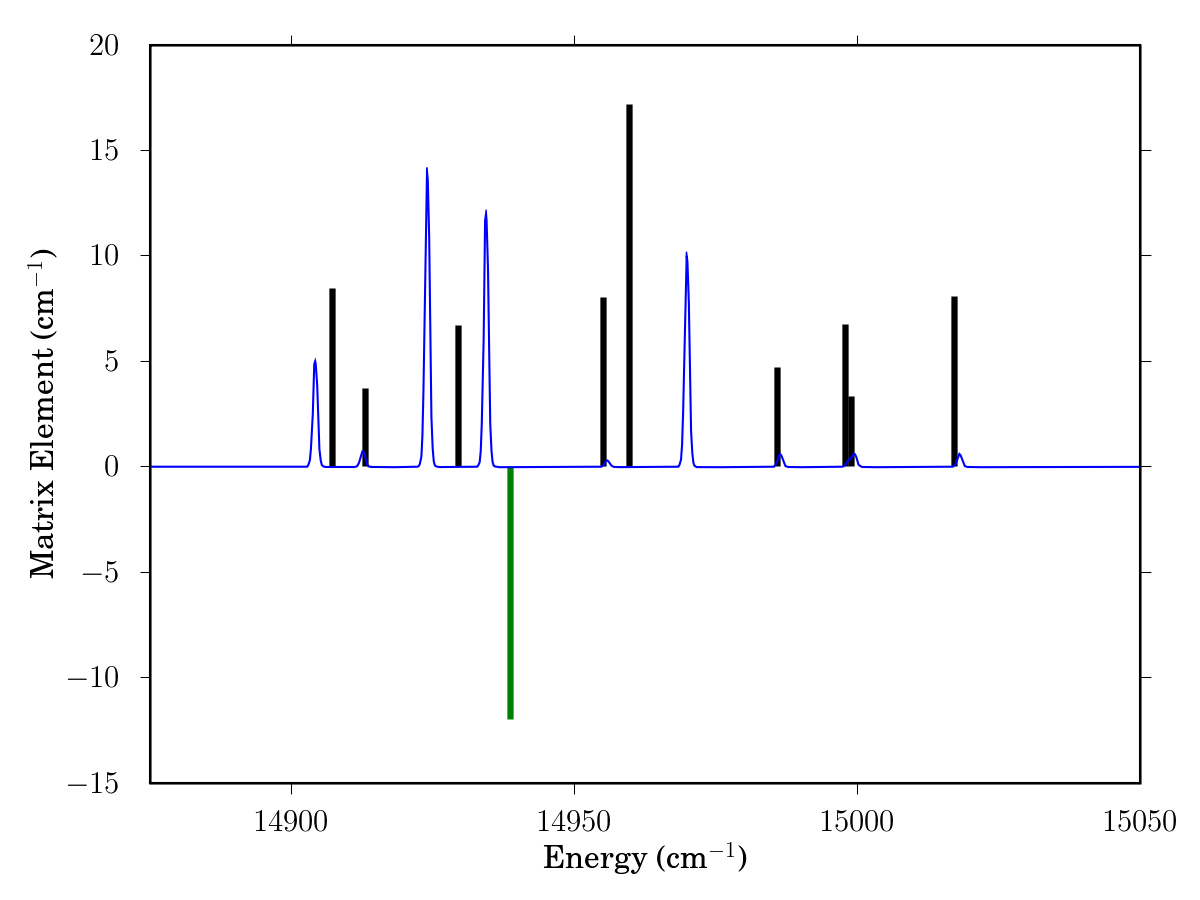
\includegraphics[width=6in]{smalley-direct.png}
\end{figure}

\begin{figure}
  \caption{Thick vertical lines: Dark basis state energies and matrix
    elements obtained by an extended LKL deconvolution of a portion of
    the \ce{NO2} spectrum reported by Smalley \emph{et. al.}
    \cite{smalley75}.  The bright state energy obtained from the first
    stage of deconvolution is displayed as a dashed vertical line in
    the positive direction, scaled to the bright$\sim$doorway matrix
    element.  The energy of the doorway state is displayed as a
    vertical line in the negative direction.  The original absorption
    spectrum is shown as a set of Gaussian lineshapes superimposed on
    the deconvolution results.  Note that the energies for the
    combined set of bright and dark states in the doorway-coupled
    basis satisfy the usual level trapping rules for dark states in a
    direct-coupled basis.}
  \label{fig:smalley-doorway}
  \centering
  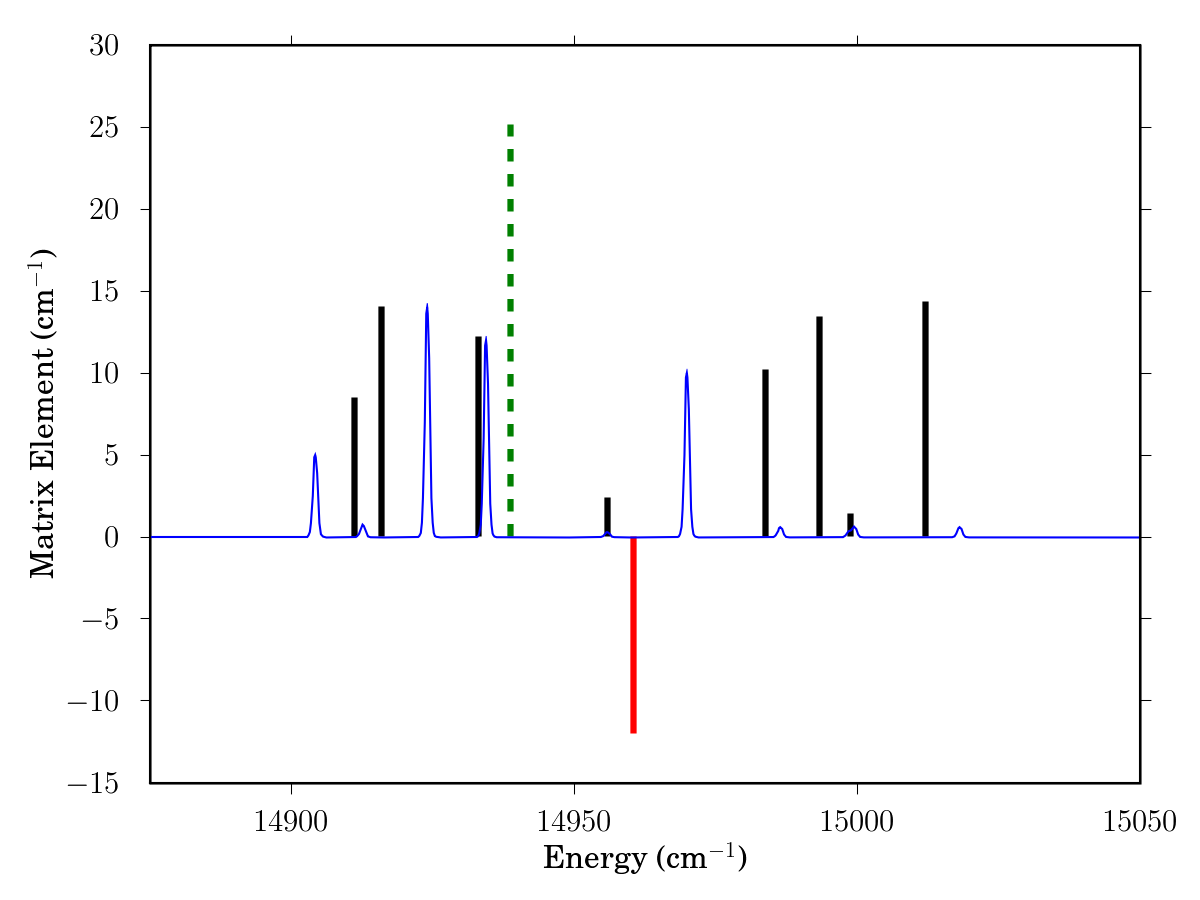
\includegraphics[width=6in]{smalley-doorway.png}
\end{figure}

This property exists for the doorway-coupling Hamiltonian because it
can be rearranged to have the same form as a direct-coupling
Hamiltonian without a matrix rotation.  Simply by re-ordering the
columns such that the bright state is embedded into the manifold of
dark states, the doorway-coupling Hamiltonian becomes identical in
form to the direct-coupling Hamiltonian.  This arrangement is shown in
Figure \ref{fig:matrix}c.  With the Hamiltonian arranged in this form,
it is clear that the distribution of doorway amplitude among the dark
states is equivalent to the distribution of bright state amplitude in
a direct-coupling model.  As a consequence, the phenomenon of level
trapping still applies to a doorway-coupled system, though the bright
state and doorway state have swapped roles.  In the doorway-coupling
Hamiltonian, the zero-order bright state and the $N-1$ zero-order dark
states are trapped between the eigenstate energies, in the same manner
as the $N$ dark states of the direct-coupling Hamiltonian.

We note in passing that doorway-coupling models with two or more
successive doorway states do not share this property.  They require a
change of basis to bring them into the ``arrowhead'' form of the
direct-coupling Hamiltonian.  In this respect, the doorway-coupling
Hamiltonian with a single doorway state is unique among the set of
doorway-coupling Hamiltonians in the spectroscopic channel basis of
Ziv and Rhodes.

To compare the discrete and continuous formulations, we have used the
methods detailed by Cable and Rhodes to re-evaluate the interaction
density spectrum for coupling to the doorway state \cite{cable80}.
Our results are presented in Figure \ref{fig:ids}; agreement with
Figure 11 of reference \cite{cable80} is within acceptable limits
given that the previous computation involved the numerical evaluation
of principal value integrals.

\begin{figure}
  \caption{Interaction density spectrum for coupling to the doorway
    state, computed from a portion of the \ce{NO2} spectrum reported
    by Smalley \emph{et. al.}  \cite{smalley75}.  These results are in
    agreement with those of Cable and Rhodes to a factor of
    proportionality (compare to their Figure 11) \cite{cable80}. }
  \label{fig:ids}
  \centering
  %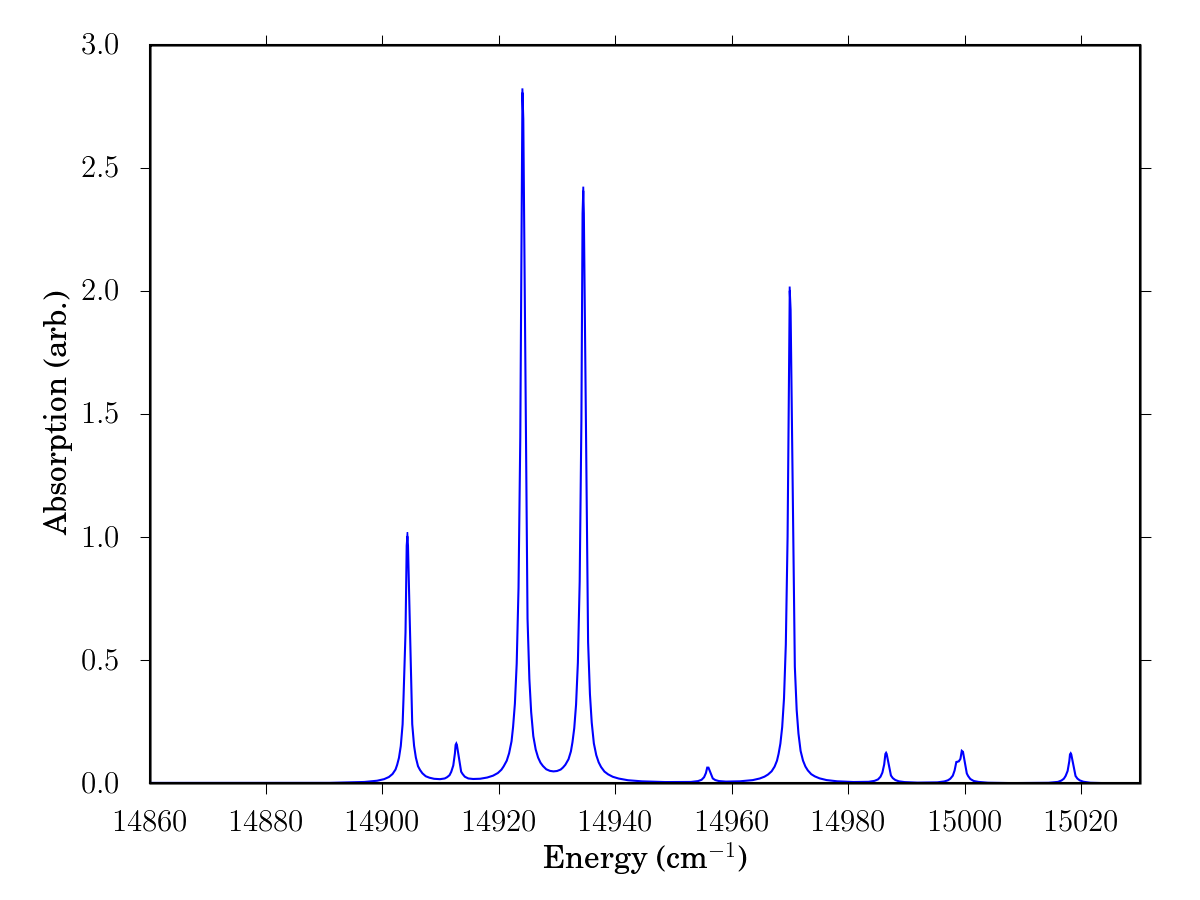
\includegraphics[width=6in]{smalley-absorption.png}
  %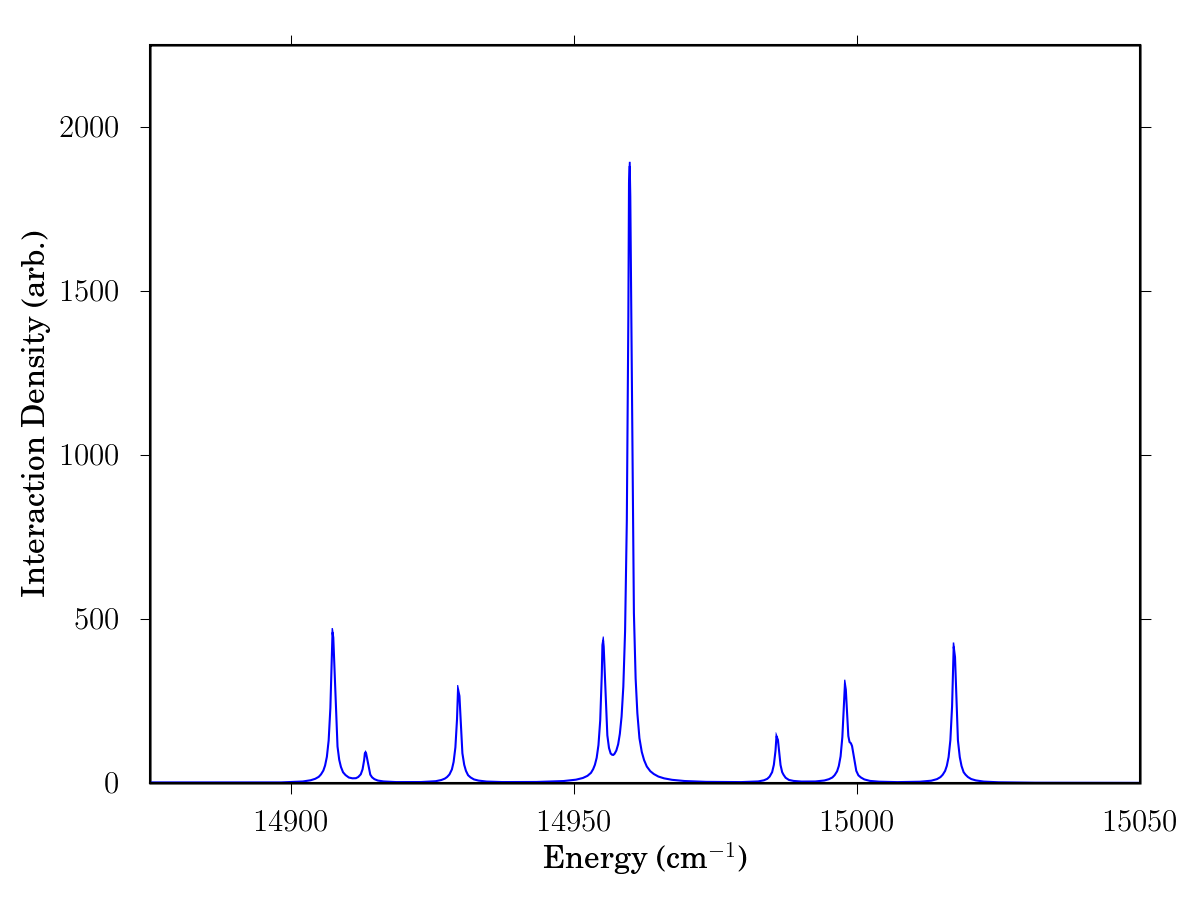
\includegraphics[width=5in]{smalley-ids0.png}
  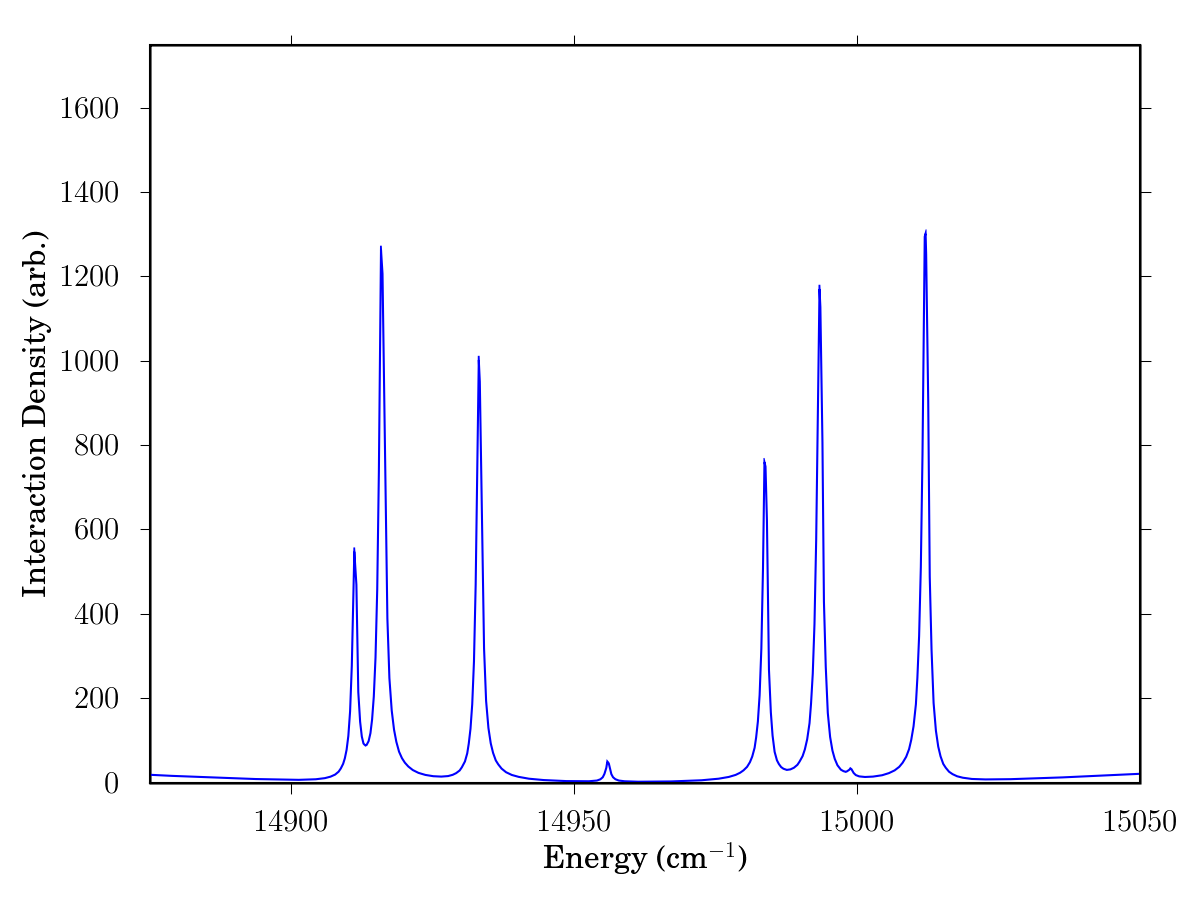
\includegraphics[width=5in]{smalley-ids1.png}
\end{figure}

Figure \ref{fig:compare-dark} compares the discrete and continuous
deconvolution results for the doorway-coupling Hamiltonian.  The
Lorentzian peaks in the interaction density spectrum coincide exactly
with the dark state energies in the discrete formulation.  Lorentzian
lineshapes transform correctly under the Hilbert transformation of
equation \ref{eq:hilbert}, producing smooth poles in the real part of
the Green's function derived from the absorption spectrum.  

\begin{figure}
  \caption{Comparison of discrete and continuous extended
    deconvolution results for the same spectrum.  The dark state
    energies and squared matrix elements in the discrete formulation
    correspond to the peaks of the interaction density spectrum in the
    continuous formulation.}
  \label{fig:compare-dark}
  \centering
  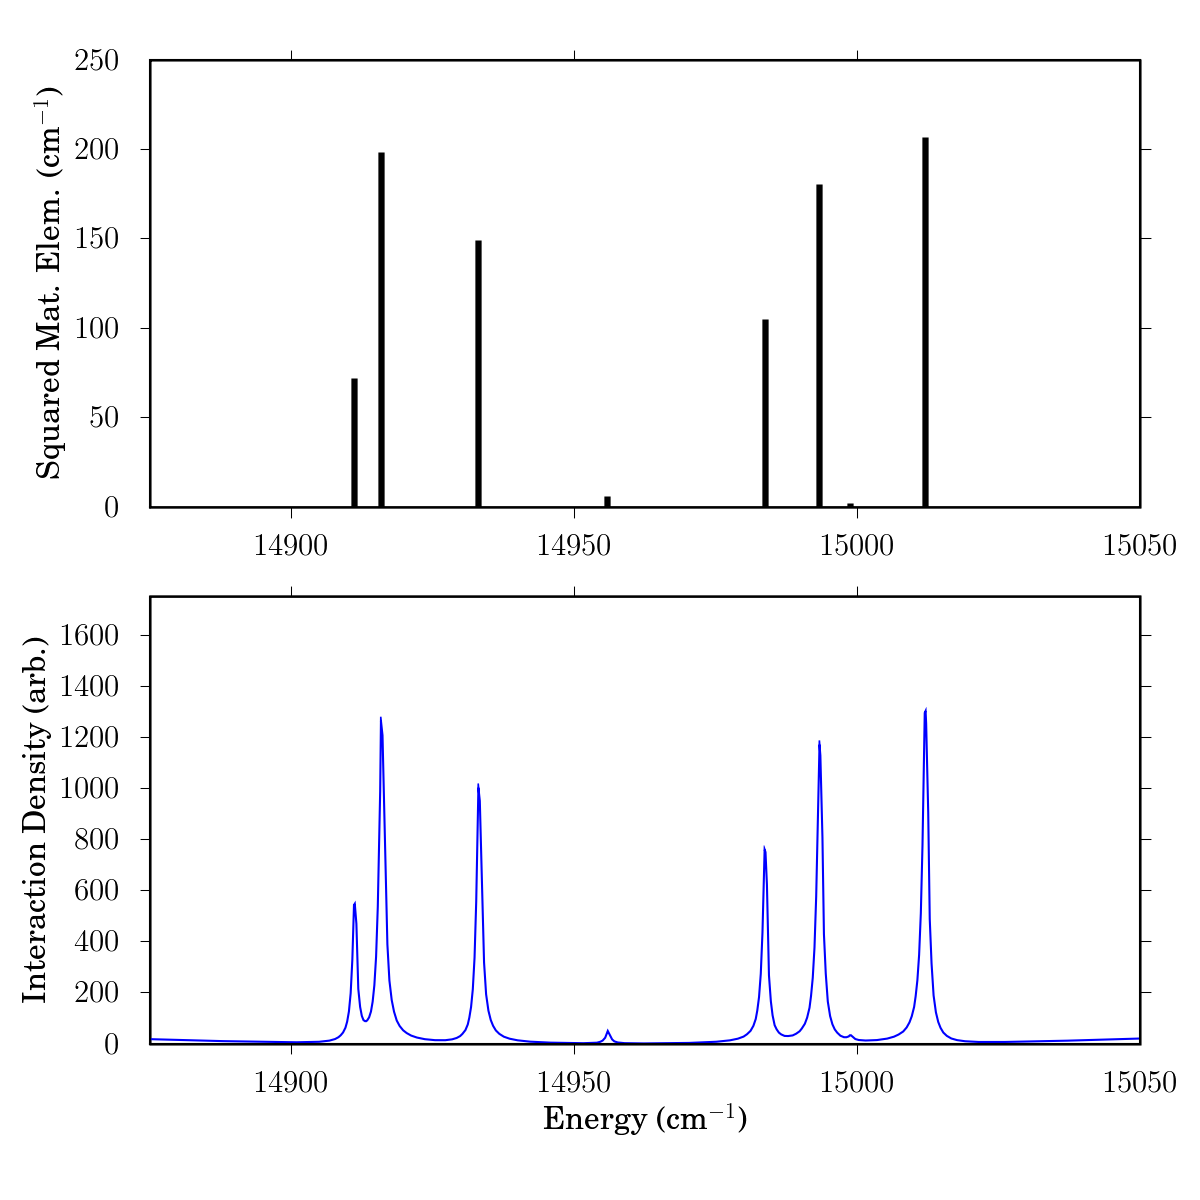
\includegraphics[width=6in]{smalley-compare-fwhm1.png}
\end{figure}

Because the continuous formulation is exact for Lorentzian lineshapes,
a continuous deconvolution of unresolved, homogeneously broadened
spectral lines will have the correct functional form, although some
peaks may remain unresolved in the resulting interaction density
spectrum.  Thus, for a spectrum with homogeneous width $\gamma$, the
interaction density spectrum $\mathcal{F}(E)$ for the doorway state is
equal to
\begin{equation}
  \mathcal{F}_{\ell}(E) = 
    \mathcal{L}_{\gamma} \; * \;
    \sum_n H_{\ell n}^2 \delta(E_n - E)
\end{equation}
where the symbol $*$ denotes convolution, $\mathcal{L}_{\gamma}$ is a
Lorentzian function with FWHM $\gamma$, and the index $m$ runs over
the diagonal block of dark states coupled to $K$.  A comparison of
discrete and continuous deconvolution results is shown in Figure
\ref{fig:broadened}, where the original discrete spectrum has been
convoluted with a Lorentzian function with a FWHM of 6 cm$^{-1}$.  The
rising wings of the interaction density spectrum arise from the
nonzero tails of the Lorentzian peaks, which cause the inverse of the
Green's function to accumulate at the edges of the computed spectrum.

\begin{figure}
  \caption{Continuous deconvolution carried out for Lorentzian
    broadened lineshapes of 6 cm$^{-1}$ fwhm, corresponding to $1/2$
    the average level spacing of the spectrum.  The continuous
    deconvolution result is consistent with the discrete result to a
    resolution of 6 cm$^{-1}$.  }
  \label{fig:broadened}
  \centering
  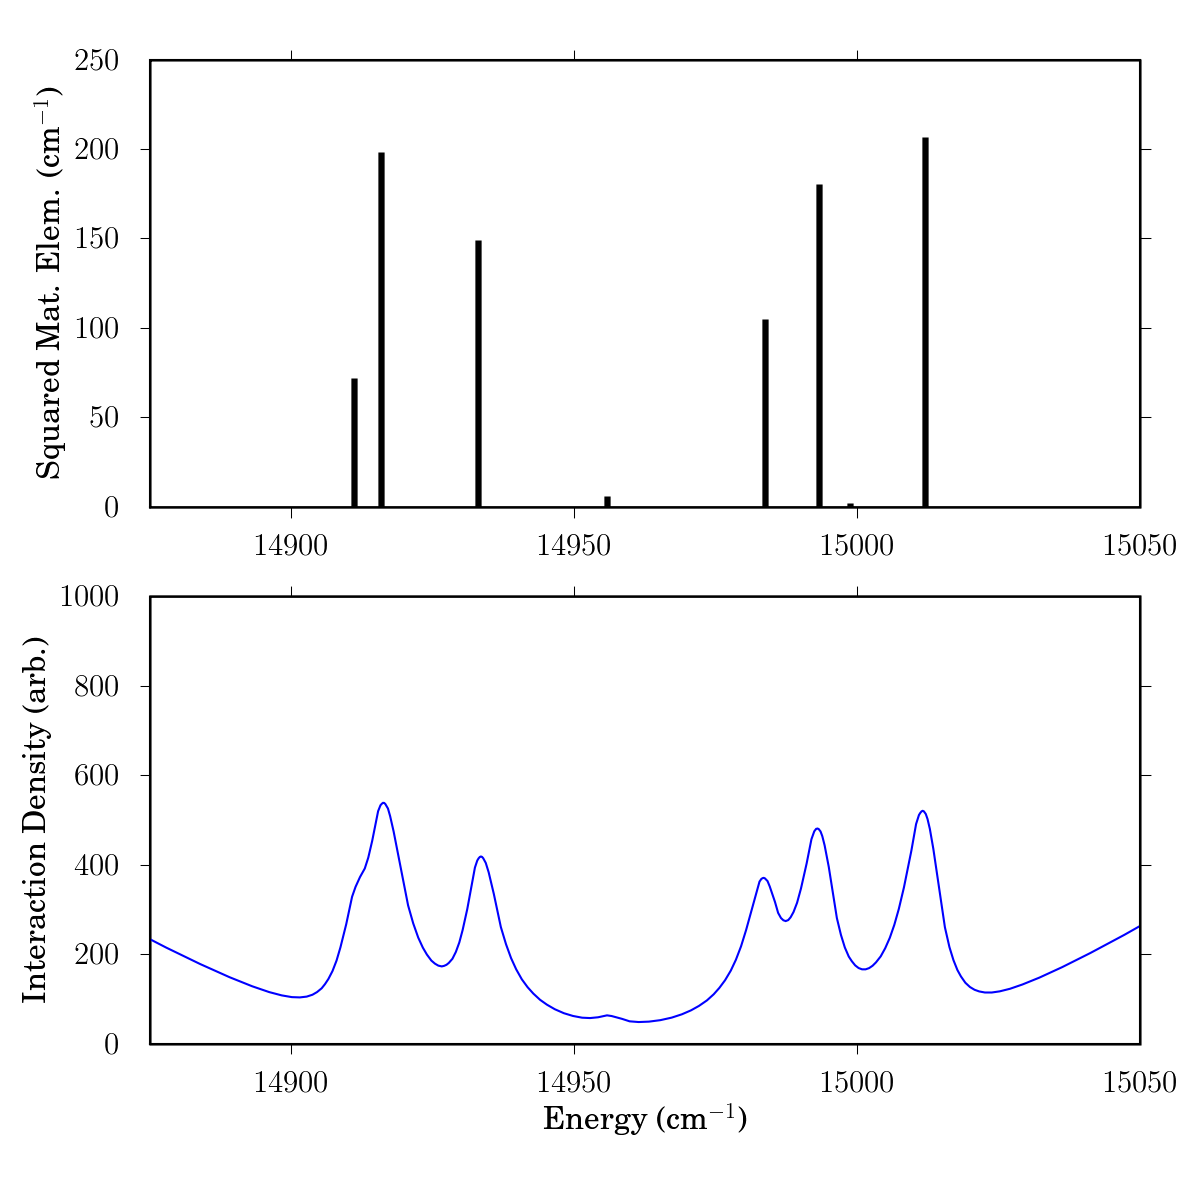
\includegraphics[width=6in]{smalley-compare-fwhm6.png}
\end{figure}

In the limit of heterogeneous broadening, the continuous form of the
deconvolution fails.  Gaussian lineshapes do not have the correct
functional form for solutions to the Green's function of equation
\ref{eq:greens-function}, and a Hilbert transformation of the spectrum
does not produce a real function with smooth poles.  If the
deconvolution procedure is carried out regardless, the resulting
interaction density spectrum will contain peaks at incorrect energies
and intensities.  In this situation, the experimentalist is faced with
two choices: discretize the spectrum and miss dark state$\sim$dark
state spacings smaller than the resolution, or convolve the spectrum
with a Lorentzian lineshape to obtain an unresolved but functionally
correct interaction density spectrum.  The parameters, $E_s$,
$H_{s\ell}^2$, and $E_{\ell}$, because they are related to moments of
the spectrum, will remain correct for any symmetric lineshape in the
spectrum.

% \section{Effects of experimental resolution, intensity noise, and
%   finite dynamic range}

% \TODO{Present Lehmann's error formulas and extend to compute errors
% for the doorway state energy and matrix element.}


% The effect of finite resolution will be to possibly miss a small
% matrix element between two dark states.  Show that this will not
% affect the positions of the bright and doorway states.  It will, by
% necessity, affect things like the next neighbor spacing distribution
% and the doorway state matrix element.

% \POINT{Evaluate Lehmann's formula for the error in the sum-of-squares of
% bright$\sim$dark matrix elements in the case that two resonances of
% equal intensity are mistaken for one resonance of twice the
% intensity.}  The error scales as the square of the energy difference
% from the bright state:
% \begin{equation}
%   \frac{\partial \sum H_{sm}^2}{\partial I_i} = 
%   \frac{(\nu_i - E_s)^2 - \sum H_{sm}^2}{\sum I_i},
% \end{equation}
% but is constant with respect to the intensity error.

% \POINT{Maybe apply gaussian noise to overlapped data, and note
%   the non-change in doorway energy and matrix element.  Use this fact
% to claim a level of robustness for the doorway information.}

% \POINT{Apply to finite dynamic range spectra.}  Since the
% doorway$\sim$bright matrix element is the sum of the $C=0$ matrix
% elements, a dynamic range of the experiment can be used to place an
% upper bound on the ``missing'' portion of this matrix element.

\section{Application to high-resolution spectra of acetylene}

In 1994, Drabbels \emph{et. al.} recorded the laser-induced
fluorescence (LIF) spectrum of the $3^3_0K^1_0$ vibronic subband of
$S_1$ acetylene at a resolution of 18 MHz \cite{drabbels94}.  The
authors used the LKL method to generate a set of direct-coupling
matrix elements from the spectral data.  However, several subsequent
investigations of this band have found strong evidence that a
single vibrational level of the $T_3$ electronic state mediates coupling
between the $S_1$ level and the remaining levels, which are classified
as high-lying vibrational levels of the $T_1$ and $T_2$ electronic
states.

Using the methods described above, we have calculated the parameters
of a doorway-coupling model Hamiltonian for each rotational level of
$3^3_0K^1_0$ reported by Drabbels \emph{et. al.}  The results are
shown in Table \ref{table:drabbels-deconv}.  Note the near-linear
change in bright state - doorway state energy difference with
increasing $J$.  This result is consistent with the observation of a
local $T_3$ vibrational level with a rotational constant slightly
different that of the singlet.

\begin{table}
  \caption{Extended deconvolution results for the $3^3_0K^1_0$
    vibrational subband of $S_1$ acetylene.  The energies of 
    the zero-order bright state, $E_s$, and doorway state, $E_{\ell}$, 
    are given, as well as the zero-order energy difference, $\Delta
    E_{s\ell}$, and bright$\sim$doorway matrix element, $H_{s\ell}$.
    All values are in units of cm$^{-1}$.}
  \label{table:drabbels-deconv}
  \centering
  \begin{tabular}{lrrrr}
    & \\
    \toprule
    & $E_s$ & $E_{\ell}$ & $\Delta E_{s\ell}$ & $H_{s\ell}$ \\
    \midrule
    %& \\
    %\multicolumn{3}{l}{$3^3_0K^1_0$}\\
    %& \\
    R(0) & 45303.1255 & 45302.8524 & -0.2731 & 0.1418 \\
    R(1) & 45305.2210 & 45305.1090 & -0.1120 & 0.1206 \\
    R(2) & 45307.1738 & 45307.2010 &  0.0272 & 0.1188 \\
    R(3) & 45308.9133 & 45309.0122 &  0.0990 & 0.1704 \\
    & \\
    Q(1) & 45300.6503 & 45300.6921 &  0.0418 & 0.1980 \\
    Q(2) & 45300.1678 & 45300.1170 & -0.0508 & 0.1245 \\
    Q(3) & 45299.4414 & 45299.2142 & -0.2272 & 0.1785 \\
    Q(4) & 45298.4825 & 45298.3072 & -0.1753 & 0.1695 \\
    \bottomrule
  \end{tabular}
\end{table}

This band of acetylene was also considered by Altunata and Field, who
derived a parameter to predict the product $E_{\ell} \times
H_{s\ell}^2$ \cite{altunata01}.  The ``skewness'' parameter of
Altunata and Field,
\begin{equation}
  S = \sum_m I_m^2 \times (E_m - E_0),
\end{equation}
is computed from the results of a single deconvolution, using the
quasi-continuous formulation of Lawrance and Knight.  The intensity
factor $I_m$ is proportional to the quantity $H_{sm}^2$ in the
discrete formulation.  The authors identify $E_0$ with the ``midpoint
of the energy axis of the L–K output.''  Because this parameter scales
with energy to the first power, it is more accurately considered an
expression for the center-of-gravity of the distribution of $\lbrace
H_{sm}^4\rbrace$ in the direct-coupling Hamiltonian.

The authors of reference \cite{altunata01} applied their $S$ parameter
to the spectrum of $3^3_0K^1_0$ reported by Drabbels \emph{et. al.}
and reported the product $E_{\ell} \times H_{s\ell}^2$ for the R(0-4)
transitions.  We compare these results with the deconvolution method
described in this work by normalizing the $S$ parameter to the
quantity $H_{s\ell}^2$, computed from the variance of the spectrum
(equation \ref{eq:doorway-moment}).  Figure \ref{fig:selen-comparison}
shows the doorway state energy computed from deconvolution and the
normalized $S$ parameter values reported in reference
\cite{altunata01}.  The small (0.03 cm$^{-1}$) discrepancies
presumably result from integration of the interaction density spectrum
(Lawrance and Knight's $B(E)$) used to compute the $S$ parameter
\cite{lawrance85}.

\begin{figure}
  \caption{Comparison between Altunata and Field's $S$ parameter and
    the bright state - doorway state energy difference ($E_s -
    E_{\ell}$) obtained from extended LKL deconvolution
    \cite{altunata01}.  To coincide with the formula for doorway state
    energy, the $S$ parameter results are scaled by the squared
    bright$\sim$doorway matrix element, which is equal to the variance
    of spectral intensity.}
  \label{fig:selen-comparison}
  \centering
  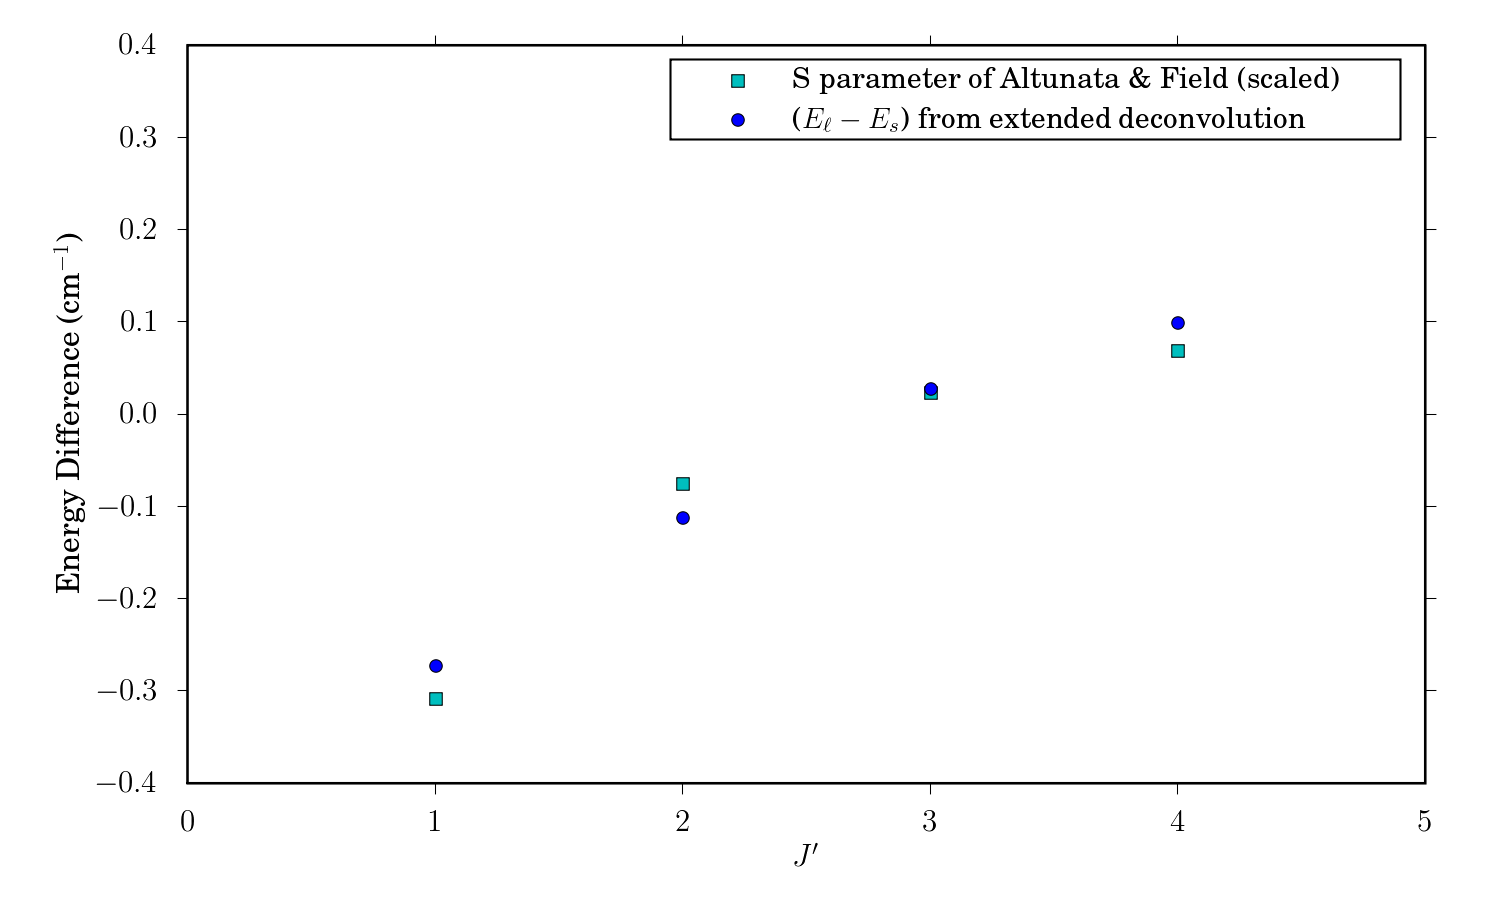
\includegraphics[width=6.5in]{selen-comparison.png}
\end{figure}

The most complete description of the doorway level in $3^3_0K^1_0$ is
given by Mishra \emph{et. al.}, who used the complimentary
spectroscopic techniques of LIF and SEELEM to record the spectrum of
long-lived states coupled weakly to $S_1$ \cite{mishra04}.  To analyze
this local $T_3$ perturber, they constructed reduced term value plots
and fit the experimental energies to a model Hamiltonian.

The results of the Hamiltonian fit by Mishra \emph{et. al.} yielded a
bright$\sim$doorway matrix element of $H_{s\ell} = 0.126$ cm$^{-1}$
for the \emph{e}-symmetry components (the authors do not give an
uncertainty for this value) \cite{mishra04}.  We compare the
deconvolution results with the Hamiltonian fit by averaging the value
of $H_{s\ell}$ obtained from extended deconvolution over the
rotational quantum number $J$.  The average bright$\sim$doorway matrix
element from deconvolution is $\langle H_{s\ell} \rangle \, = \, 0.138
\pm 0.021$ cm$^{-1}$, in agreement with the previous results.  The
bright state and doorway state energies obtained from deconvolution
are compared to the reduced term values of reference \cite{mishra04}
in Figure~\ref{fig:ryan-comparison}.  As expected, the deperturbed
energies lie between the nominal $S_1$ and $T_3$ eigenstate
energies inferred from the spectrum.

\begin{figure}
  \caption{The $S_1$ and $T_3$ basis state energies obtained from
    extended LKL deconvolution are shown together with the reduced
    term values of Mishra \emph{et. al.} \cite{mishra04}.  Top:
    $e$-symmetry basis state energies obtained from R-branch
    transitions.  Bottom: $f$-symmetry basis state energies obtained
    from Q-branch transitions. The deperturbed energies from
    deconvolution lie between the nominal $S_1$ and $T_3$ eigenstate
    energies inferred from the spectrum.}
  \label{fig:ryan-comparison}
  \centering
  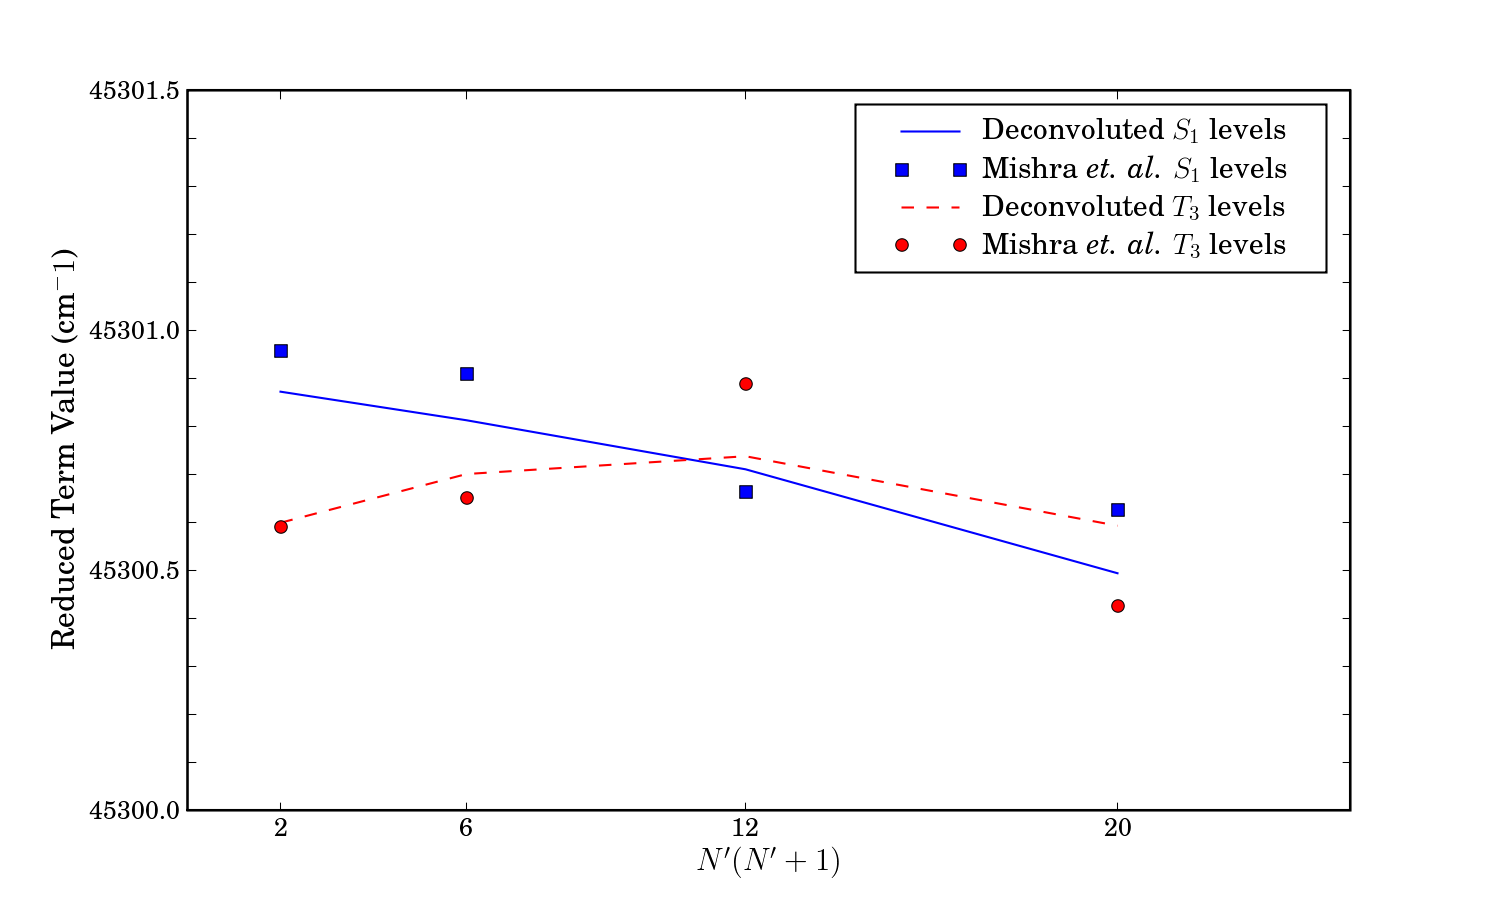
\includegraphics[width=6.5in]{ryan-comparison-r.png}
  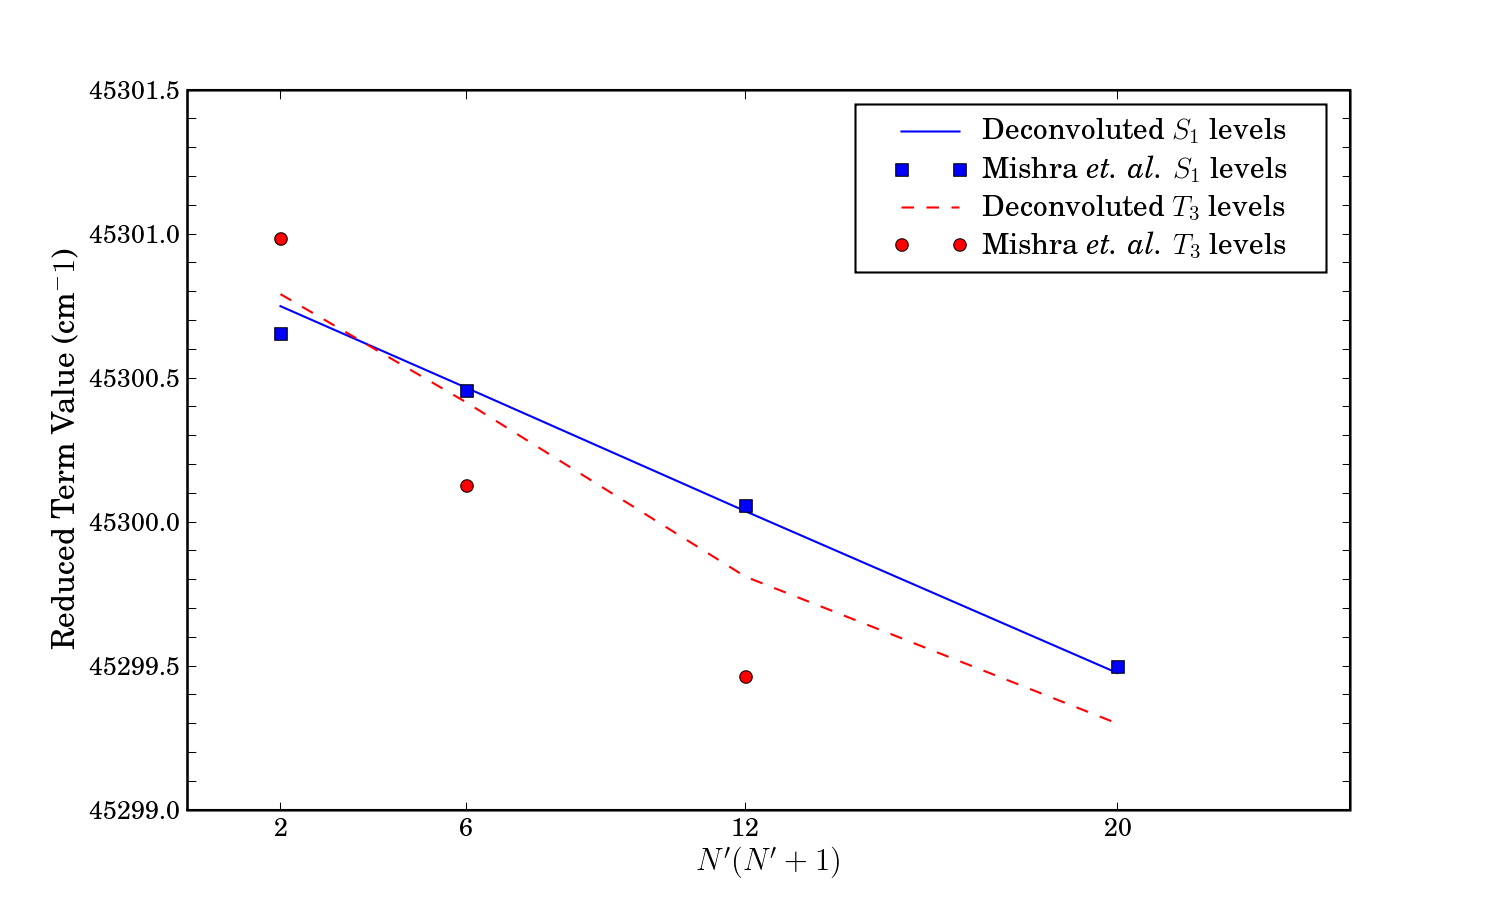
\includegraphics[width=6.5in]{ryan-comparison-q.png}
\end{figure}

The use of LIF intensities in the deconvolution procedure instead of
absorption intensities rests on the assumption that only the bright
state character of an eigenstate contributes to the fluorescence
intensity.  This is indeed the case for the low-lying triplet basis
states of acetylene, from which transitions to the ground state are
spin-forbidden.  
% (If the assumption of no fluorescence from dark basis
% states not hold completely, errors arising from dark state ``leakage''
% are described in the appendix of reference \cite{delon95}.)

\section{Conclusion}

We have shown how to extend established methods of spectral
deconvolution to uniquely determine the parameters of a
doorway-coupling effective Hamiltonian.  The most important parameters
of the effective Hamiltonian, the doorway state energy and
bright$\sim$doorway matrix element, were related to simple moments of
the spectral intensity distribution.  By making a correspondence to
the work of Ziv and Rhodes on continuous deconvolution, we have shown
how the parameters that define an effective Hamiltonian can be derived
for any number of sequential doorway states.

This technique was applied to the spectrum of the $3\nu_3$ $K=1$
vibrational level of $S_1$ acetylene, where a single, local, $T_3$
doorway level mediates coupling to the $T_{1,2}$ manifold.  The
deperturbed $T_3$ energies and matrix elements were shown to be
consistent with past studies.  A comparison was made to the $S$
parameter of Altunata and Field, which is equal to the product
$E_{\ell} \times H_{s\ell}^2$.



%\bibliography{deconv}
% \bibliography{master}
% \bibliographystyle{plain}
% \end{document}
% LocalWords:  deperturbation Intramolecular IVR intersystem deperturb occurrs
% LocalWords:  rovibronic Hamiltonians Lorentzian eigenvectors vibronic
% LocalWords:  perturber
